\begin{figure}[thpb]
  \centering
  %\begin{tikzpicture}
    %\clip [rounded corners=1em] (0,0) rectangle coordinate (centerpoint) (5,7.5cm);
%    \node[minimum width=\linewidth,minimum height=174pt,draw=black,rounded corners=1em,fill=bgcolor,draw=black]
%    {};
%    \node[name=img] {
      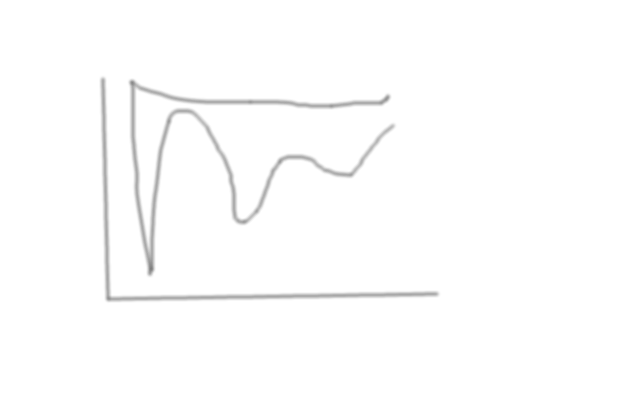
\includegraphics[width=0.93\columnwidth]{./pix/tmp.png}
      
\includegraphics{./qrcode/qrcode-staticwalking.png}\\
      Video: http://danlofaro.com/phd/staticwalking/
%    };
%    \draw [bgcolor, rounded corners=1em, line width=1em,inner sep=0pt]
%    (img.north west) --
%    (img.north east) --
%    (img.south east) --
%    (img.south west) -- cycle
%    ;
%  \end{tikzpicture}
\caption{Hubo static walking using Hubo-Ach as the primary controller.  The static walking algorithm was implimented by Youngbum Jun.  All control was
implimented using Daniel M. Lofaro's Hubo-Ach system.
}
  \label{fig:staticwalking}
\end{figure}
